\documentclass{article}

% if you need to pass options to natbib, use, e.g.:
\PassOptionsToPackage{numbers, compress}{natbib}
% before loading neurips_2023

% to compile a camera-ready version, add the [final] option, e.g.:
\usepackage[final]{neurips_2023}

\usepackage[utf8]{inputenc} % allow utf-8 input
\usepackage[T1]{fontenc}    % use 8-bit T1 fonts
\usepackage{hyperref}       % hyperlinks
\usepackage{url}            % simple URL typesetting
\usepackage{booktabs}       % professional-quality tables
\usepackage{amsfonts}       % blackboard math symbols
\usepackage{nicefrac}       % compact symbols for 1/2, etc.
\usepackage{microtype}      % microtypography
\usepackage{xcolor}         % colors
\usepackage{amsmath}
\usepackage{amssymb}
\usepackage{graphicx}
\usepackage{array}
\usepackage{colortbl}
\usepackage{pifont}
\usepackage{tikz}
\usetikzlibrary{arrows.meta,positioning,calc}
\graphicspath{{./figures/iclr/}{./figures/rep/}{./figures/}{./images/}}

% -- light helpers (no template variation) --
\definecolor{rowhi}{HTML}{EAF1FC}
\definecolor{goodbg}{HTML}{E3F5E9}
\definecolor{badbg}{HTML}{FBE7E7}
\definecolor{vitc}{HTML}{1F4E9B}
\definecolor{swinc}{HTML}{B5651D}
\definecolor{effc}{HTML}{2E7D32}
\newcommand{\cmark}{\textcolor{effc}{\ding{51}}}
\newcommand{\xmark}{\textcolor{red!65!black}{\ding{55}}}
\newcommand{\gcell}{\cellcolor{goodbg}}
\newcommand{\rcell}{\cellcolor{badbg}}
\newcommand{\F}{\text{F1}}
% playing-card family markers
\newcommand{\hand}{\textcolor{effc}{$\clubsuit$}}   % handcrafted features
\newcommand{\img}{\textcolor{vitc}{$\diamondsuit$}} % image / CNN / transformer
\newcommand{\seq}{\textcolor{swinc}{$\heartsuit$}}  % sequence / RNN

\title{99\% Sure? Gabor Begs to Differ:\\
A Time-Frequency Look at Parkinson's Handwriting\\
and a Structure-Preserving Image Encoding}

\author{%
  Andrea Porcelli \\
  Department of Computer Science \\
  University of Bari Aldo Moro \\
  Bari, Italy \\
  \texttt{a.porcelli34@studenti.uniba.it}
}

\begin{document}
\maketitle

\begin{abstract}
Detecting Parkinson's disease (PD) from handwriting is a clinically useful and
difficult problem. PaHaW is a public benchmark of online handwriting from $72$
subjects ($37$ with PD, $35$ healthy controls) recorded on a graphics tablet;
reported accuracies on it are typically high, often above $90\%$. We study how much
of this performance is supported once the data are evaluated carefully. The PD
signature is a time-frequency phenomenon, a $4$-$6$\,Hz tremor interleaved with
sub-decisecond pen arrests, and the Gabor uncertainty principle
($\sigma_t\sigma_f\!\ge\!\nicefrac{1}{4\pi}$) limits how well any fixed representation
can resolve both at once on a short, $150$\,Hz signal. We (i) review the PaHaW
literature and the evaluation choices that can inflate reported scores; (ii) give a
time-frequency argument that the task is not yet resolved; and (iii) rather than
separating the PD and healthy signals (an ill-posed inverse problem), re-encode the
kinematics into a structure-preserving colour image that a frozen Vision Transformer
reads. Under repeated nested cross-validation with the Nadeau-Bengio corrected
$t$-test, our best encoding is above chance and above a clinical baseline
(F1 $0.7457$ vs.\ $0.5080$, $p=0.0187$), but no encoding is statistically separable from its
closest rivals. The recovered signal is modest, and the fine-grained ranking is not
resolvable at this cohort size.
\end{abstract}

\section{Introduction}
\label{sec:intro}
Online handwriting is an attractive, non-invasive biomarker for Parkinson's disease:
a tablet records the pen trajectory and pressure while the patient draws, and the
trace carries the motor signature of the disease, a $4$-$6$\,Hz tremor, reduced and
more variable velocity, micrographia, and brief akinetic arrests
\citep{drotar2016,impedovo2019}. A decade of surveys has charted the field
\citep{impedovo2019review,vessio2019,destefano2019,aouraghe2023}, and methods range
from handcrafted kinematic descriptors to convolutional, recurrent, and reservoir
deep models \citep{pereira2018,gallicchio2018,diaz2021}. PaHaW \citep{drotar2016} is the standard public benchmark: online handwriting from
$72$ subjects ($37$ with PD, $35$ controls) on a Wacom tablet. Reported accuracies on
it are high, routinely above $90\%$ and sometimes $98$-$100\%$. These figures are
encouraging; we ask how much survives a careful evaluation.

We find that part of this performance is fragile, for two reasons. The first is
\emph{statistical}: on $72$ subjects, leakage between train and test, single splits,
and naive significance tests across correlated folds all push reported accuracy above
what generalizes. The second is \emph{physical}: the PD signature is a
time-frequency phenomenon, and the Heisenberg-Gabor uncertainty principle limits
how sharply any \emph{fixed} representation can localize the tremor in frequency and
the arrests in time at the same instant. A kinematic feature vector, a spectrogram
with one window, or a wavelet bank with one quality factor all commit, before seeing
the data, to one point on this trade-off; on a few-second recording at $150$\,Hz that
commitment cannot resolve both regimes, so such a score can be optimistic.

This paper (1)~reviews the PaHaW literature and the evaluation choices that can
inflate scores (Sec.~\ref{sec:lit}); (2)~gives a time-frequency argument that the
task is not yet resolved (Sec.~\ref{sec:theory}); and (3)~rather than separating the
PD and healthy signals (an ill-posed inverse problem), re-encodes the kinematics into
a structure-preserving colour image read by a frozen Vision Transformer
(Sec.~\ref{sec:method}). Evaluated carefully (Sec.~\ref{sec:results}), it clears
chance and a clinical baseline but nothing finer.

\section{The PaHaW Literature and Its Evaluation Pitfalls}
\label{sec:lit}
We do not attempt an exhaustive survey. Instead we select a few well-known works that
are widely cited as state of the art on PaHaW and that, taken together, represent the
main methodological pillars of the field (Table~\ref{tab:comparison}). Read side by
side, they share four recurring evaluation pitfalls.

\paragraph{Subject leakage.}
Each PaHaW writer contributes up to eight task recordings. When recordings are
pooled, augmented, or held out one at a time, the same patient can appear in train
and test, and a classifier may recognize the writer rather than the disease. Shin et
al.\ \citep{shin2025} report $99.98\%$ under leave-one-out, but leave out a single
recording while the patient's other seven stay in training. Group-aware splitting
(subject $=$ group) is the standard defense \citep{varma2006}, and we enforce it.

\paragraph{Feature-selection bias.}
Choosing features or hyper-parameters on the full dataset before splitting inflates
results. Valla et al.\ \citep{valla2022} measured this on PaHaW Task~1: non-nested
feature selection reports $84.86\%$, the nested variant $73.71\%$, an $11.15$-point
gap from selecting on test data alone.

\paragraph{High performance through feature explosion.}
A related route to inflated scores is dimensionality: extracting hundreds of
descriptors from a few dozen subjects. Shin et al.\ \citep{shin2025} derive $944$
in-air dynamics features for $\sim\!75$ subjects; with so many degrees of freedom a
model can fit the cohort almost perfectly, and combined with non-nested selection
this can produce near-ceiling accuracies that need not generalize.

\paragraph{No uncertainty, no valid test.}
None of the cited works reports a standard deviation or confidence interval; on our
$72$ subjects the fold-to-fold F1 standard deviation reaches $0.21$
(Sec.~\ref{sec:results}), so a point estimate can coincide with a lucky fold. Tests,
when present, are naive paired $t$-tests across folds, which are anti-conservative
because folds share training data. Notably, the two studies that nest their selection
(Valla's nested variant and ours) land near $0.74$, while the headline figures
cluster near $0.99$.

\begin{table}[t]
\caption{Selected representative works on PaHaW (best Task~1 result, or the
task-merged headline). Family: \hand~handcrafted, \img~image/CNN, \seq~sequence/RNN.
The four audit columns mark nested selection (Nest), freedom from feature-selection
bias (FS), subject-disjoint splits (Subj), and reported variability (Var):
\cmark~yes, \xmark~no, $\sim$ unclear. ($\ast$ task-level LOO; $\S$ single hold-out;
n/r not reported.)}
\label{tab:comparison}
\centering
\small
\setlength{\tabcolsep}{5.5pt}
\renewcommand{\arraystretch}{1.15}
\begin{tabular}{@{}cllcccccc@{}}
\toprule
 & Method & Validation & Acc. & F1 & Nest & FS & Subj & Var \\
\midrule
\hand & Drot\'ar et al.\ \citep{drotar2016}        & 10-fold (tasks 2-8) & 0.8130 & 0.8400$^\sim$ & \xmark & \xmark & \cmark & \xmark \\
\hand & Impedovo \citep{impedovo2019}              & 10-fold                 & 0.9840 & n/r           & \xmark & \xmark & \cmark & \xmark \\
\hand & Valla et al.\ \citep{valla2022} (non-nest.)& 10-fold                 & 0.8490 & 0.8491        & \xmark & \xmark & \cmark & \xmark \\
\hand & Valla et al.\ \citep{valla2022} (nested)   & nested 10-fold          & 0.7371 & 0.7300$^\sim$ & \cmark & \cmark & \cmark & \xmark \\
\seq  & Diaz et al.\ \citep{diaz2021}              & 10-fold                 & 0.9375 & n/r           & \xmark & \xmark & \cmark & \xmark \\
\img  & Wang et al.\ \citep{wang2024bspc}          & 5-fold (augmented)      & 0.8470 & 0.8570        & \xmark & \xmark & $\sim$ & \xmark \\
\seq  & Kumar \& Ghosh \citep{kumar2024}           & $3{:}1$ hold-out         & $1.0000^\S$ & n/r      & \xmark & \xmark & $\sim$ & \xmark \\
\hand & Shin et al.\ \citep{shin2025}              & LOOCV$^\ast$            & 0.9860 & 0.9860        & \xmark & \xmark & \xmark & \xmark \\
\midrule
\rowcolor{rowhi}
\img & \textbf{Ours} (effort, ViT, RF) & nested $3{\times}10$-fold & 0.7524 & 0.7457 & \cmark & \cmark & \cmark & \cmark \\
\bottomrule
\end{tabular}
\end{table}

\section{A Time-Frequency Limit on the Task}
\label{sec:theory}

\paragraph{The signal.}
PaHaW records the pen at $f_s=150$\,Hz. The disease superimposes two phenomena at very
different scales. The first is the Parkinsonian \emph{tremor}: an involuntary
oscillation of the hand, clinically a rest/postural tremor, whose frequency is
$4$-$6$\,Hz, i.e.\ the pen position and pressure oscillate $4$ to $6$ times per
second. It is a \emph{narrow-band} event one wants to localize in frequency. The
second is a set of aperiodic pen-lifts and akinetic \emph{arrests} of tens of
milliseconds, \emph{broadband} impulses one wants to localize in time. A spiral lasts
a few seconds, so the tremor contributes only a handful of cycles.

\paragraph{The window dilemma (STFT).}
The short-time Fourier transform analyses $x[n]$ through a window $w$ of length $L$,
\begin{equation}
X[m,k]\;=\;\sum_{n} x[n]\,w[n-mH]\,e^{-j2\pi kn/L},
\qquad
\Delta t \approx \frac{L}{f_s},\quad \Delta f \approx \frac{f_s}{L}.
\label{eq:stft}
\end{equation}
The window length $L$ sets \emph{both} resolutions at once, with product
$\Delta t\,\Delta f \approx 1$ fixed: a long window resolves frequency but smears the
arrests, a short one times the arrests but blurs the tremor. Separating $4$ from
$6$\,Hz needs $\Delta f\lesssim 2$\,Hz, hence
\begin{equation}
L \;\gtrsim\; \frac{f_s}{\Delta f} \;\approx\; \frac{150}{2} \;=\; 75~\text{samples}
\;\approx\; 0.5~\text{s},
\label{eq:wall}
\end{equation}
during which any sub-decisecond arrest is washed out. No single $L$ serves both
regimes.

\paragraph{The wavelet dilemma.}
The continuous wavelet transform replaces the fixed window with dilations of a mother
wavelet $\psi$,
\begin{equation}
W[a,b]\;=\;\frac{1}{\sqrt{a}}\sum_{n} x[n]\,\psi^{*}\!\Big(\frac{n-b}{a}\Big),
\qquad
Q \;=\; \frac{f}{\Delta f}\;=\;\text{const}.
\label{eq:cwt}
\end{equation}
The window now shrinks with scale, which suits handwriting better, but the quality
factor $Q$ and the shape of $\psi$ are fixed before training: the wavelet \emph{moves}
the commitment along the bound rather than removing it.

\paragraph{The bound.}
Both transforms obey the Heisenberg-Gabor uncertainty principle: a signal cannot be
arbitrarily sharp in time and frequency at once. For any analysis atom with
time spread $\sigma_t$ and frequency spread $\sigma_f$,
\begin{equation}
\sigma_t\,\sigma_f \;\ge\; \frac{1}{4\pi},
\label{eq:gabor}
\end{equation}
with equality only for the Gabor atom, a Gaussian-modulated sinusoid. Concretely, to
pin the tremor to $\pm1$\,Hz one must integrate over $\sigma_t\gtrsim 0.08$\,s, longer
than an arrest; to time an arrest to $\pm10$\,ms one must accept
$\sigma_f\gtrsim 8$\,Hz, wider than the tremor band. The two goals are in direct
conflict, and \eqref{eq:gabor} fixes the exchange rate.

\paragraph{The limit is upstream of the model.}
The decisive point is that \eqref{eq:gabor} constrains the \emph{input}, not the
classifier. Figure~\ref{fig:blackbox} makes it concrete: whatever sits in the black
box, a random forest on handcrafted features, an RNN, a CNN, or our own encoder, it
receives a short $150$\,Hz recording whose joint time-frequency content is already
limited. The tremor-versus-arrest ambiguity is a property of the measurement, not of
the network, so however powerful the model, it cannot recover information the input
never contained. A model can be at most as sharp as its input allows; it cannot cheat
the physics. The competing feature sets of the literature are competing guesses about
where to lose information, none breaks the bound, and a reported $99\%$ therefore need
not mean the signal is resolved, only that the evaluation was permissive.

\begin{figure}[t]
\centering
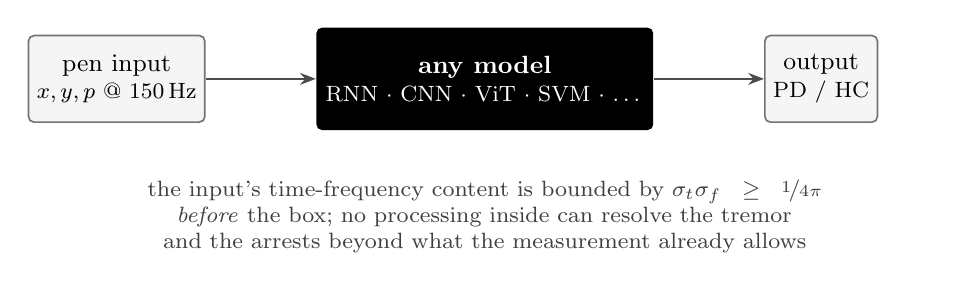
\begin{tikzpicture}[font=\small, node distance=10mm,
  io/.style={rounded corners=2pt, draw=black!55, line width=0.6pt, fill=black!4,
    minimum height=11mm, align=center, inner sep=3pt},
  ar/.style={-{Stealth[length=2mm]}, line width=0.9pt, draw=black!70}]
\node[io] (in) {pen input\\[-1pt]\footnotesize $x,y,p$ @ $150$\,Hz};
\node[rounded corners=2pt, fill=black, text=white, minimum height=13mm,
      minimum width=42mm, align=center, right=14mm of in] (box)
  {\textbf{any model}\\[-1pt]\footnotesize RNN $\cdot$ CNN $\cdot$ ViT $\cdot$ SVM $\cdot$ \ldots};
\node[io, right=14mm of box] (out) {output\\[-1pt]\footnotesize PD / HC};
\draw[ar] (in) -- (box);
\draw[ar] (box) -- (out);
\node[anchor=north, font=\footnotesize, text=black!75, text width=0.92\textwidth, align=center]
  at ($(box.south)+(0,-5mm)$)
  {the input's time-frequency content is bounded by $\sigma_t\sigma_f\ge\nicefrac{1}{4\pi}$
   \emph{before} the box; no processing inside can resolve the tremor and the arrests
   beyond what the measurement already allows};
\end{tikzpicture}
\caption{The uncertainty bound is upstream of the classifier. Independently of what
fills the black box, the pen-to-decision map inherits a time-frequency resolution
limit set by the input alone. The difficulty of PaHaW is a property of the
measurement, not of the model.}
\label{fig:blackbox}
\end{figure}

\section{Method: a Structure-Preserving Colour Encoding}
\label{sec:method}

\paragraph{Dataset and what we train on.}
PaHaW \citep{drotar2016} contains $72$ subjects, $37$ with PD and $35$ healthy
controls, recorded on a Wacom Intuos tablet sampling the pen at $f_s=150$\,Hz. Each
sample is a $7$-tuple
\begin{equation}
s_n=\big(\,x_n,\;y_n,\;t_n,\;b_n,\;p_n,\;\theta^{\mathrm{az}}_n,\;\theta^{\mathrm{al}}_n\,\big),
\end{equation}
the pen position $(x,y)$, timestamp $t$, contact status $b\in\{0,1\}$ (on-surface vs.\
in-air), axial pressure $p$, and pen azimuth $\theta^{\mathrm{az}}$ and altitude
$\theta^{\mathrm{al}}$. From the on-surface samples we derive the kinematics: velocity
$v_n=\lVert(x_{n+1}{-}x_n,\,y_{n+1}{-}y_n)\rVert/\Delta t$, acceleration
$a_n=(v_{n+1}{-}v_n)/\Delta t$, and \emph{effort} $e_n=v_n p_n$ (a motor-load proxy);
together with pressure and the two geometric angles, these are the signals we colour
onto the trajectory. Every subject performs eight tasks; we use Task~1, the
Archimedean spiral, so each subject contributes one recording and the subject-level
decision coincides with the recording-level one, removing the cross-task leakage that
inflates other studies.

\paragraph{Representations.}
We render ten image modalities of the spiral. Six are single-signal maps that colour
the trajectory by one channel with a perceptually uniform colormap (velocity,
acceleration, pressure, azimuth, altitude, effort); three are RGB triplets that pack
three channels into the colour planes (\texttt{rgb\_vpa}, \texttt{rgb\_vpe},
\texttt{rgb\_vpz}); and one is the raw uncoloured stroke, a geometry-only control.
Each image is embedded by one of three frozen ImageNet-pretrained backbones (ViT-B/16
\citep{dosovitskiy2021vit}, Swin-T \citep{liu2021swin}, EfficientNet-B0
\citep{tan2019efficientnet}), $z$-scored, and classified by a per-fold-tuned head
(logistic regression, three SVMs, a random forest, two MLPs). The baseline is the
$33$-d handcrafted clinical vector of Drot\'ar et al.\ \citep{drotar2016} and
Impedovo \citep{impedovo2019} (kinematic and pressure statistics, timing, geometry,
and $4$-$6$/$0$-$2$\,Hz band power). In all, $31$ inputs ($10$ modalities $\times$ $3$
backbones $+$ baseline) $\times\,7$ heads $=217$ cells.

\paragraph{Why re-encode instead of separate.}
Learning a filter that separates the PD signal from the healthy one is ill-posed at
this resolution and cohort size. We change the question: instead of separating, we
\emph{preserve}. Drawing the trajectory on a $224\times224$ canvas and colouring each
point by a kinematic channel is a quantization that records \emph{how fast},
\emph{how hard}, and \emph{where} the pen moved, discarding only the fine phase that
\eqref{eq:gabor} says we could not have recovered. The encoding keeps the structure
that distinguishes a slow, tremulous, high-pressure spiral from a healthy one, and
lifts a one-dimensional signal into the two-dimensional input that large-scale visual
pretraining is optimized for. This is the dual advantage: it sidesteps the resolution
wall and lets us transfer a frozen encoder a $72$-subject cohort could never train
(Fig.~\ref{fig:pipeline}).

\begin{figure}[t]
\centering
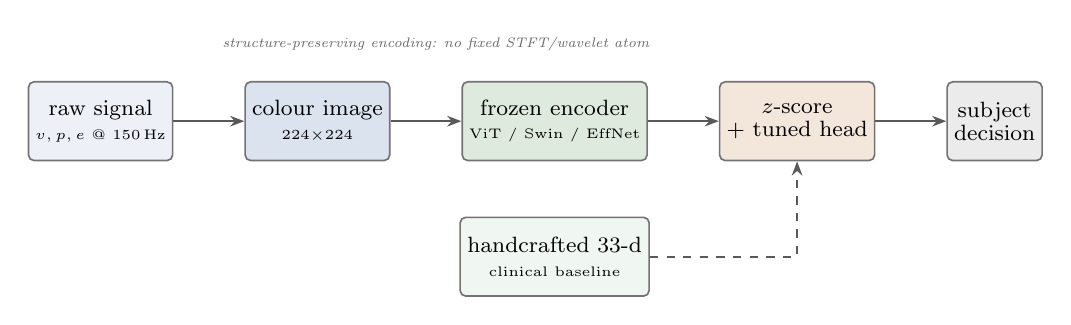
\begin{tikzpicture}[font=\footnotesize, node distance=7mm and 9mm,
  box/.style={rounded corners=2pt, draw=black!55, line width=0.6pt,
    minimum height=10mm, align=center, inner sep=2.5pt},
  ar/.style={-{Stealth[length=1.8mm]}, line width=0.7pt, draw=black!65}]
\node[box, fill=vitc!8] (s) {raw signal\\[-1pt]\tiny $v,p,e$ @ $150$\,Hz};
\node[box, fill=vitc!16, right=of s] (i) {colour image\\[-1pt]\tiny $224{\times}224$};
\node[box, fill=effc!16, right=of i] (e) {frozen encoder\\[-1pt]\tiny ViT / Swin / EffNet};
\node[box, fill=swinc!16, right=of e] (h) {$z$-score\\[-1pt] $+$ tuned head};
\node[box, fill=black!8, right=of h] (d) {subject\\[-1pt] decision};
\foreach \a/\b in {s/i,i/e,e/h,h/d}\draw[ar] (\a)--(\b);
\node[box, fill=effc!7, below=7mm of e, minimum width=24mm] (b){handcrafted $33$-d\\[-1pt]\tiny clinical baseline};
\draw[ar, dashed] (b.east) -| (h.south);
\node[anchor=south, font=\itshape\tiny, text=black!60] at ($(i.north)!0.5!(e.north)+(0,2.6mm)$){structure-preserving encoding: no fixed STFT/wavelet atom};
\end{tikzpicture}
\caption{The pipeline. The raw kinematics are re-encoded as a colour image (a
structure-preserving quantization), embedded by a frozen backbone, and classified by
a per-fold-tuned head. The handcrafted vector (dashed) bypasses the encoder.}
\label{fig:pipeline}
\end{figure}

\section{Evaluation}
\label{sec:results}

\paragraph{Protocol.}
We use $R=3$ repeats (seeds $42,43,44$) of $10$-fold \texttt{StratifiedGroupKFold},
$N=30$ test folds per cell; an inner $3$-fold grid search tunes every head on the
training portion only. Models are compared with the Nadeau-Bengio corrected
resampled paired $t$-test \citep{nadeau2003}, which repairs the optimistic variance
of the naive fold-wise test by accounting for train/test overlap:
\begin{equation}
t_{\text{NB}}=\frac{\bar d}{\sqrt{\big(\tfrac{1}{N}+\tfrac{n_\text{test}}{n_\text{train}}\big)s^2}},
\qquad \text{df}=N-1,
\label{eq:nb}
\end{equation}
which for $10$-fold CV multiplies the naive variance by $0.144/0.033\approx4.3$, so
$t_{\text{NB}}$ is $\sim\!2.1\times$ smaller than its naive twin.

\begin{table}[t]
\caption{Champion ($=$ effort, ViT, RF; mean F1 $\mathbf{0.7457}$) vs.\ rivals, naive
and Nadeau-Bengio corrected paired $t$-tests (df$=29$). The F1 column is each row
model's \emph{own} mean F1 over the $30$ folds (mean AUC in the AUC row), not a
difference. \rcell{}red $=$ naive-significant, \gcell{}green $=$ survives correction.
Backbone marker: \img~ViT, \seq~Swin. The correction turns the $7$ ``significant''
verdicts here into $0$; over all $30$ rivals, $29$ into $10$.}
\label{tab:sig}
\centering
\small
\setlength{\tabcolsep}{5.5pt}
\renewcommand{\arraystretch}{1.1}
\begin{tabular}{@{}clccccc@{}}
\toprule
 & Comparison & F1 & $t_{\text{naive}}$ & $p_{\text{naive}}$ & $t_{\text{NB}}$ & $p_{\text{NB}}$ \\
\midrule
\img & velocity, ViT, RF        & 0.7090 & 1.36 & 0.1850 & 0.65 & 0.5194 \\
\seq & raw, Swin, RF            & 0.6473 & 2.43 & \rcell 0.0215 & 1.17 & 0.2527 \\
\img & acceleration, ViT, MLP-s & 0.6372 & 3.53 & \rcell 0.0014 & 1.69 & 0.1010 \\
\img & rgb\_vpa, ViT, RF        & 0.6235 & 2.73 & \rcell 0.0106 & 1.31 & 0.1999 \\
\seq & rgb\_vpz, Swin, MLP-f    & 0.6230 & 2.70 & \rcell 0.0114 & 1.30 & 0.2046 \\
\img & rgb\_vpz, ViT, RF        & 0.6226 & 4.02 & \rcell 0.0004 & 1.93 & 0.0631 \\
\seq & rgb\_vpe, Swin, MLP-f    & 0.6184 & 3.18 & \rcell 0.0035 & 1.53 & 0.1378 \\
\seq & pressure, Swin, MLP-f    & 0.6157 & 3.32 & \rcell 0.0025 & 1.59 & 0.1221 \\
\midrule
     & handcrafted baseline (RF) & 0.5080 & n/a & $<$0.0001 & 2.49 & \gcell $\mathbf{0.0187}$ \\
     & champion F1 vs.\ chance   & 0.7457 & n/a & $<$0.0001 & 3.64 & \gcell $\mathbf{0.0011}$ \\
     & champion AUC vs.\ chance  & 0.7972 & n/a & $<$0.0001 & 4.11 & \gcell $\mathbf{0.0003}$ \\
\bottomrule
\end{tabular}
\end{table}

\paragraph{What survives.}
The best encoding is \emph{effort} on ViT-B/16 with a random forest:
F1~$=0.7457{\scriptscriptstyle\,\pm.18}$, AUC~$=0.7972{\scriptscriptstyle\,\pm.19}$,
accuracy~$=0.7524{\scriptscriptstyle\,\pm.16}$ over $30$ folds. It is significantly
above chance on every metric (corrected $p\le0.0011$) and above the $33$-feature
clinical baseline (F1 $0.7457$ vs.\ $0.5080$, corrected $p=0.0187$; Table~\ref{tab:sig}).
This is the part of the signal the theory predicts: \emph{which} channel we encode
matters, and effort and velocity, which carry the tremor and its pressure modulation,
are the ones that help.

\paragraph{What does not.}
Nothing finer is resolvable. Against its $30$ rivals the winner is significantly
better for $29$ under a naive test but for only $10$ under the correction, and for
none of its nine nearest competitors (Table~\ref{tab:sig}). The fold-to-fold spreads overlap
almost completely: below the effort/velocity pair the ranking is flat down to the
handcrafted baseline, and subject-level F1 is discrete (only $9$ distinct values over
the $\sim\!7$ held-out subjects of a fold). The best head even flips
between random forest (F1) and MLP (AUC~$=0.7976$) with the metric, and the modal
tuned hyper-parameter wins only $48\%$ of folds on average. The picture is
two-sided: the encoding recovers a real but coarse signal, effort/velocity $>$
handcrafted $>$ chance, while the fine-grained ranking is not resolvable at this
cohort size. This suggests PaHaW is not yet a solved task, and that very high
reported figures may partly reflect evaluation choices.

\section{Conclusion}
The PD signature is a time-frequency object no fixed representation can resolve, by
the Heisenberg-Gabor principle, so PaHaW's high reported figures may partly reflect
leakage and optimistic testing rather than a fully solved task. Rather than separate
the two signals, we re-encode them into a structure-preserving colour image a frozen
vision model can attack; evaluated honestly it clears chance and a clinical baseline
but nothing finer. On $72$ subjects, the honest number is a modest one.

\paragraph{Reproducibility.}
Splits use fixed seeds $\{42,43,44\}$; the sweep, corrected test, and figures are
produced by standalone scripts (\texttt{run\_repeated.py}, \texttt{nadeau\_bengio.py},
\texttt{full\_pairwise.py}).

\small
\bibliographystyle{plainnat}
\bibliography{references}

\end{document}
